\documentclass[runningheads]{llncs}
\usepackage[T1]{fontenc}

\usepackage[table]{xcolor}

\usepackage{booktabs}
%\usepackage[square,sort,comma,numbers]{natbib}
\usepackage[pdfstartview=XYZ,
bookmarks=true,
colorlinks=true,
linkcolor=blue,
urlcolor=blue,
citecolor=blue,
pdftex,
bookmarks=true,
linktocpage=true, % makes the page number as hyperlink in table of content
hyperindex=true
]{hyperref}

\usepackage{rotating} % Rotating table
\usepackage{subcaption}
\usepackage{graphicx}
\usepackage{multirow}
\usepackage{amsmath}


\title{Generating Synthetic Data Is Complicated: Know Your Data and Know Your Generator}
\titlerunning{Generating Synthetic Data Is Complicated}

\author{Jonathan Latner\inst{1}\orcidID{0000-0002-1825-0097} \and
Marcel Neunhoeffer\inst{1,2}\orcidID{0000-0002-9137-5785}  \and
J\"{o}rg Drechsler\inst{1,2,3}\orcidID{0009-0009-5790-3394}}

\authorrunning{Latner et al.}


\institute{Institute for Employment Research, Nuremberg, Germany 
\email{\{jonathan.latner, marcel.neunhoeffer,joerg.drechsler\}@iab.de} \and
Ludwig-Maximilians-Universit\"at, Munich, Germany \and
University of Maryland, College Park, USA
}



\begin{document}

\maketitle 

\begin{abstract}

In recent years, more and more synthetic data generators (SDGs) based on various modeling strategies have been implemented as Python libraries or R packages. With this proliferation of ready-made SDGs comes a widely held perception that generating synthetic data is easy.  We show that generating synthetic data is a complicated process that requires one to understand both the original dataset as well as the synthetic data generator.  We make two contributions to the literature in this topic area.  First, we show that it is just as important to pre-process or clean the data as it is to tune the SDG in order to create synthetic data with high levels of utility. Second, we illustrate that it is critical to understand the methodological details of the SDG to be aware of potential pitfalls and to understand for which types of analysis tasks one can expect high levels of analytical validity.

\keywords{Synthetic \and Utility \and CTGAN \and DataSynthesizer \and synthpop}
\end{abstract}

\section{Introduction}

The idea of synthetic microdata\footnote{Throughout the paper, when we refer to data, we are referring to classical microdata (i.e., one observation per individual unit), as opposed to summary tables or images.} for statistical disclosure limitation was introduced more than 30 years ago \cite{rubin1993statistical,little1993statistical,liew1985data} and has become increasingly popular in recent years \cite{jordon2022synthetic,drechsler202330}. The general appeal of synthetic data is obvious: synthetic data promises to mimic the statistical properties of the original data while maintaining the confidentiality of individual records. In practice, releasing synthetic data means fitting a model to the original data and then generating new data based on this model.\footnote{Note that there are different philosophies about the definition of original data and how much pre-processing (e.g., dealing with missing values or outliers) one should do to the original data before data synthesis depending on the synthesis goals (replacement of the original data vs. tool for preparing to work with the original data in a safe environment). In section \ref{sec:know_your_data} we describe the data and any pre-processing steps in detail.} The new interest in synthetic data was spurred by the development of new methods and algorithms to generate synthetic data, many of which are available as open-source software packages, see, e.g., \cite{nowok2016synthpop,ping2017datasynthesizer,ctgan}. 

This leaves the general impression that generating synthetic data has become easy and that software libraries offer a one size fits all solution. While it is indeed easy (even for novices) to generate synthetic data, it is hard to generate high-quality data. This paper addresses the question: What makes generating high-quality synthetic data hard? In particular, we focus on the data one wants to synthesize and the synthetic data generators (SDG) one wishes to use. We show that one must possess both good knowledge of the data and the generator when deciding which SDG might be appropriate for what data. 

\section{Study design}\label{sec:study_design}

In this study, we illustrate the complications in generating high quality synthetic data with limited knowledge of the data and/or the generator.  To do so, we use one dataset (SD2011) and three different SDGs  (CTGAN, DataSynthesizer, and synthpop). We emphasize that the goal of this paper is explicitly not to compare the performance of the three synthesizers. The SDGs we use have already been extensively compared and contrasted in previous papers \cite{dankar2021fake,little2022comparing}. We only use these synthesizers to illustrate our point that knowledge of the data and of the synthesizer are key to obtain high utility synthetic datasets.  We use three utility measures: pMSE and computational run-time (as defined in Appendix \ref{appendix:utility_measures}) as well as one-way frequency tables to compare the graphical distribution of variables for the synthetic and original data.  Replication code is available on GitHub.\footnote{\url{https://github.com/jonlatner/KEM_GAN/tree/main/latner/projects/comparison}}

\subsection{Data}

The data we use are called Social Diagnosis 2011 - Objective and Subjective Quality of Life in Poland (SD2011) and are included as part of the synthpop package, but are also publicly available.\footnote{ \url{http://www.diagnoza.com/index-en.html}}  The data comprise $35$ variables and $5000$ observations, $21$ variables are categorical, and $14$ variables are continuous.

The reason why we use SD2011 data is that it contains many properties of real data, including missing values, outliers, `messy' values, and generated variables.  Previous evaluations used clean data from Census \cite{little2022comparing} or machine learning benchmarks (Kaggle, UCI, OpenML) \cite{dankar2021fake}.  Clean or even simulated data can be valuable, especially for evaluation purposes, but real data present challenges for SDGs that are not otherwise understood.  For example, some SDGs cannot be used on data with missing values.  Therefore, the ability to synthesize missing values is a stage of development that SDGs must go through before they can be applied to real data.\footnote{Early versions CTGAN could not be used on data with missing values (\url{https://github.com/sdv-dev/CTGAN/issues/39}).}  

\subsection{Synthetic data generators (SDGs)}

{\bf synthpop} (Version 1.8.0) \cite{nowok2016synthpop} is an \textsf{R} package that implements parametric and ML based models (classification and regression trees (CART) and random forests) to generate synthetic data. In our application we use the default settings of the package.\footnote{Default means that CART models are used for synthesis with complexity parameter = 0.001 (smaller values will grow larger trees), and minbucket = 5 (the minimum number of observations in any terminal node).} synthpop follows a sequential process, where the first variable to be synthesized is generated by drawing new values from the marginal distribution of this variable (either by drawing from a parametric distribution or by sampling from the empirical distribution), and the subsequent variables are synthesized one at a time, always conditioning on those variables that have been synthesized in earlier steps. 

{\bf DataSynthesizer} (Version 0.1.13) \cite{ping2017datasynthesizer} is a Python package that implements the PrivBayes algorithm \cite{zhang2017privbayes}.  PrivBayes is designed to address the challenges associated with a differentially private method for releasing synthetic data outputs from high-dimensional real data inputs.  To do this, the package implements a Bayesian network model to estimate the joint distribution of the data.  

To generate synthetic data from a Bayesian network, the first step is to specify a graphical model (a directed acyclical graph (DAG)) that represents how and in what way the different variables are related to each other. DataSynthesizer doesn't require this model structure as input, instead it tries to estimate the optimal structure given the data. As a hyperparameter users can set the maximum number of parents ($k$) that should be considered for the model. The more parents, the more complex relationships between the variables. After specifying the model and estimating its parameters from the original data, synthetic data are generated by sampling new values based on the probabilities from the model's conditional probability table.  

For example, imagine data with four columns (variables) with categorical values: age (young, middle, old), education (less than secondary, secondary, and more than secondary), gender (M and F), and income (low, middle, and high).   The number of observations (or rows) are not relevant because the data are transformed into a frequency table with one cell for each unique combination of groups.  In this example, there are 54 cells  ($3 \times 3 \times 2\times 3$).  If we assume that age, education, and gender are the parents of income, then each value in the conditional probability table represents the conditional probability of each income category given the states of the other three variables. The algorithm calculates the probabilities based on the frequencies from all possible combinations of the variables.  To make this model tractable for high dimensional data, the graph structure enforces conditional independence between some of the variables, reducing the number of parameters that need to be estimated. Once the model is defined and parameters are estimated, the Bayesian network generates synthetic data by sampling  new values using the estimated probabilities.  In our applications, We use default settings except for the number of parents, which we set to $k=2$ (default is "greedy", which means that DataSynthesizers tries to find the optimal value for $k$). 

{\bf CTGAN} (Version 1.9.0) \cite{ctgan} is a Python package that is part of the Synthetic Data Vault (SDV) package \cite{patki2016synthetic}.  In their original application, generative adversarial networks (GANs) were designed to create synthetic images  \cite{goodfellow2014generative}, but the approach was later adapted to also create synthetic microdata \cite{park2018data}.  GANs simultaneously train two neural networks: a generator and a discriminator. The goal of the generator is to create synthetic data that becomes increasingly indistinguishable from original data.  The goal of the discriminator is to get better at distinguishing between original and synthetic data.  This adversarial process goes back and forth until the discriminator cannot distinguish between the original data and the generated data.  

To illustrate how GANs generate synthetic data, imagine we have one variable: income (LN) from Census data with a mean of 10 and a standard deviation of 1.  First, the generator network receives random noise vectors as input, typically sampled from a standard normal distribution with mean of 0 and a standard deviation of 1, and sends it to the discriminator to be evaluated.  Second, the discriminator evaluates the synthetic data alongside real data to determine the probability that the generated data is real (1) or fake (0).  If the discriminator determines that the generated data are fake, it sends feedback to the generator in the form of a loss function.  Higher values indicate that it is easier for the discriminator to differentiate between real and fake data.  Third, the generator then updates its parameters based on the loss function and the learning rate, which determines the magnitude of this update.  The higher the learning rate, the larger the adjustments the generator will make to its parameters in response to the feedback.  Fourth,  updated data generated from the updated parameters are sent to the discriminator.  Ultimately, this back and forth process results in a generator that produces synthetic data that ideally has the same statistical properties as the original data.  
In our application we mostly rely on default settings except for the number of epochs which we set to 600 (default is 300), but we also vary a number of other hyperparameters, as we explain in detail below.  

\section{Know your data}\label{sec:know_your_data}

SD2011 contain a variety of characteristics found in real data that can present a challenge to synthetic data generators (SDGs). These challenges should be addressed prior to applying a SDG.  However, cleaning the data requires knowledge of the data that is not always available to those with knowledge of a given SDG and may not be easy to detect or follow simple rules.  We use DataSynthesizer ($k=2$) to demonstrate the importance of preprocessing the data, but the points raised in this section are applicable to all SDGs.

{\bf Missing values.} In real data, missing values are sometimes coded as either negative values or large positive values (999999).  For example, in the variable \texttt{wkabdur} (Months working abroad in 2007-2011) from SD2011, 97.5\% of all values are -8.  The interpretation is values of -8 represent missing values and only 2.5\% of the units contained in the sample worked abroad between 2007 and 2011.  If these values are not cleaned and coded as missing before applying the SDG or the SDG is informed that these values represent missing values (which is possible for example in synthpop), then the SDG will treat these values as regular values to be included in the synthetic data, which will reduce statistical utility.  For example, if we did not code values of -8 as missing in the original data, then values between -8 and 0 would be created in the synthetic data that do not exist in the original data, as shown in Figure \ref{fig:graph_datasynthesizer_wkabdur}.  

\begin{figure}[t]
    \centering        
    \resizebox{.8\textwidth}{!}{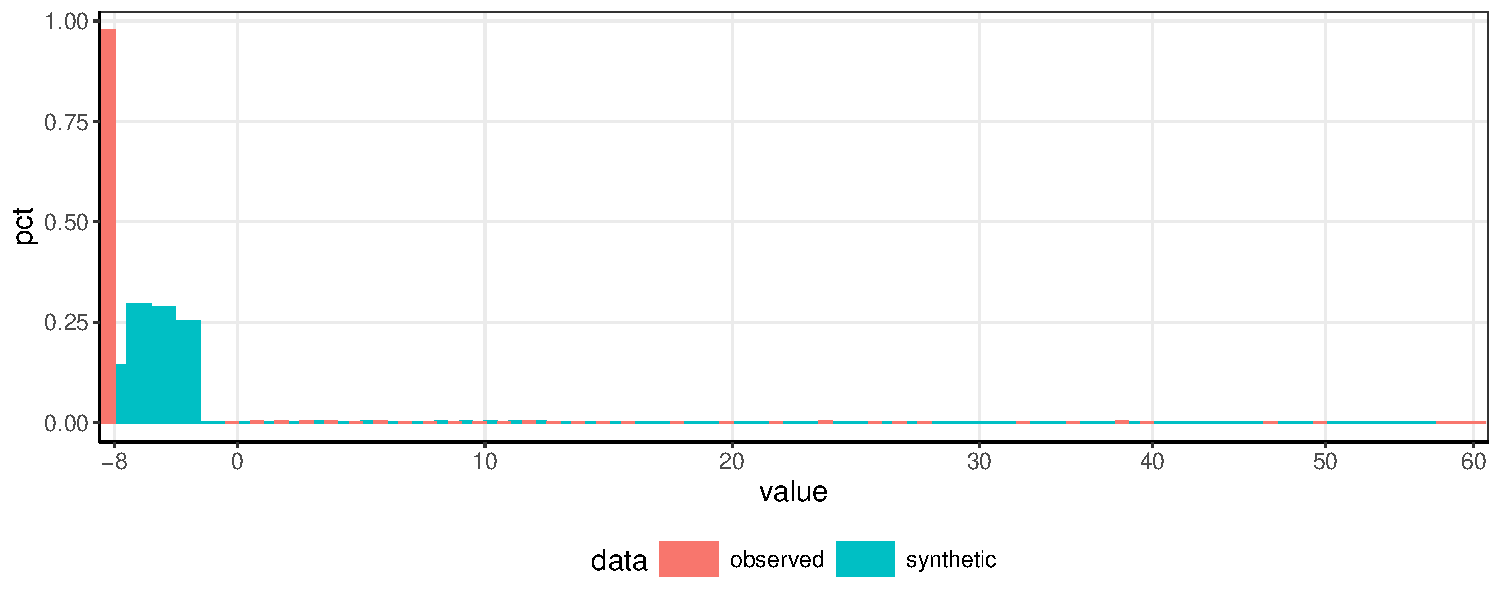
\includegraphics{../graphs/datasynthesizer_wkabdur.pdf}}
    \caption{The encoding of missing values is important. In this example, missing values of a numeric variable (on the x-axis are the values of the variable "Work abroad duration (in weeks)") were encoded as $-8$. If these negative values are treated as numeric when generating the synthetic data other (meaningless) negative values can be created. In red we display the distribution of values in the original data, in blue the distribution of values in the synthetic data.}\label{fig:graph_datasynthesizer_wkabdur}
    \vspace{-2em}
\end{figure}

{\bf Generated variables.} Generated variables are variables that are deterministic functions of other variables included in the dataset.  In SD2011, there are two generated variables.  The variable \texttt{agegr} is generated from \texttt{age} by classifying the age variable into 6 age groups and the variable \texttt{bmi} is generated from the variables \texttt{height}(cm) and \texttt{weight}(kg) (\texttt{bmi}=\texttt{weight}/$(\texttt{height}/100)^2$).  

It is not necessary to synthesize generated variables and doing so can be problematic as inconsistencies might arise in the synthetic data.  For example, in the case of \texttt{agegr}, if we apply the SDG to the original data that still includes \texttt{agegr}, then some synthetic values of \texttt{agegr} would be inconsistent with the synthetic values of \texttt{age}. In Figure \ref{fig:graph_datasynthesizer_frequency_agegr_errors} the frequency of the age groups derived from the synthetic \texttt{age} variable are shown for each category of \texttt{agegr} (frequencies are based on $m=5$ synthetic datasets). We drop values that match so the graph only shows the mismatches.  For example, for synthetic observations classified in age group 25-34 according to \texttt{agegr}, 165 (0.66\%) observations have a generated synthetic age between 16-24 and 279 (1.12\%) have a generated synthetic age between 35-44.  In total, 7.88\% of all observations would be misclassified.

To avoid these inconsistencies, generated variables should be dropped prior to applying the SDG, and then recreated based on the synthetic values of the underlying variables. However, one needs to be aware of the problem to avoid it. In practical situations, logical constraints between the variables can be much more difficult to identify and it requires good knowledge of the data to avoid implausibilities that subject matter experts would easily detect. 

\begin{figure}[t]
    \centering        
    \resizebox{.8\textwidth}{!}{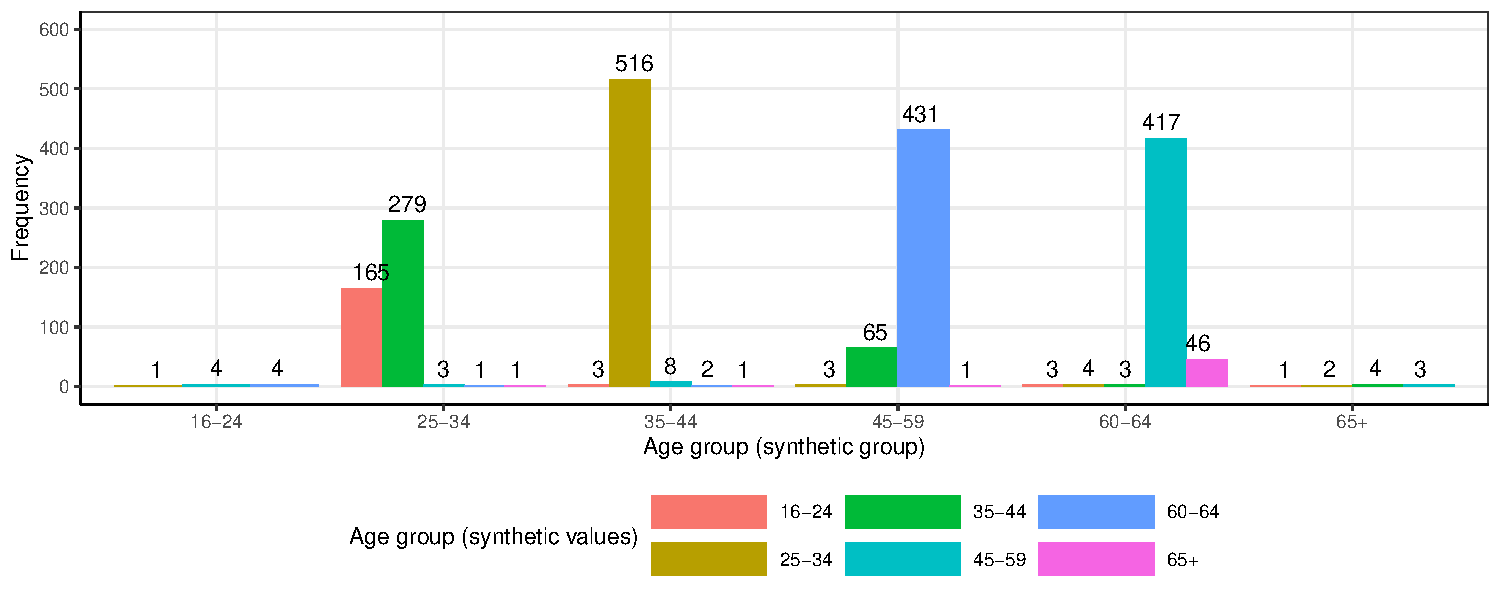
\includegraphics{../graphs/datasynthesizer_frequency_agegr_errors.pdf}}
    \caption{Synthesizing variables generated variables, i.e., variables that are deterministic functions of other variables, can lead to inconsistencies in the synthetic data. Here, the generated variable synthetic age group is not always consistent with the synthetic age values, i.e., DataSynthesizer misclassified some observations. }\label{fig:graph_datasynthesizer_frequency_agegr_errors}
    \vspace{-2em}
\end{figure}

{\bf Outliers.} Outliers can cause problems if they are not modeled carefully. For example, in the case of \texttt{bmi}, there is an outlier value of 450 in the original data.  While this value is an obvious error,\footnote{The record with a BMI of 450 has \texttt{height} (cm) = 149 and \texttt{weight} (kg) = NA.  If we calculate weight from bmi and height, then weight equals 999 or one metric ton.} what would be the implications if it were correct (and thus could not simply be removed before the synthesis)?  If we included the value of 450 in the original data, then some SDGs would create values between 450 and 76 in the synthetic data that do not exist in the original data, as shown in Figure \ref{fig:graph_datasynthesizer_bmi}.  Fortunately, in our case, \texttt{bmi} is a generated variable, which we can drop.  However, the example serves to illustrate that the existence of outlier values can affect the ability of SDGs to create synthetic data with high levels of utility and might also be problematic from a privacy perspective.  


\begin{figure}[t]
    \centering        
    
    \resizebox{.8\textwidth}{!}{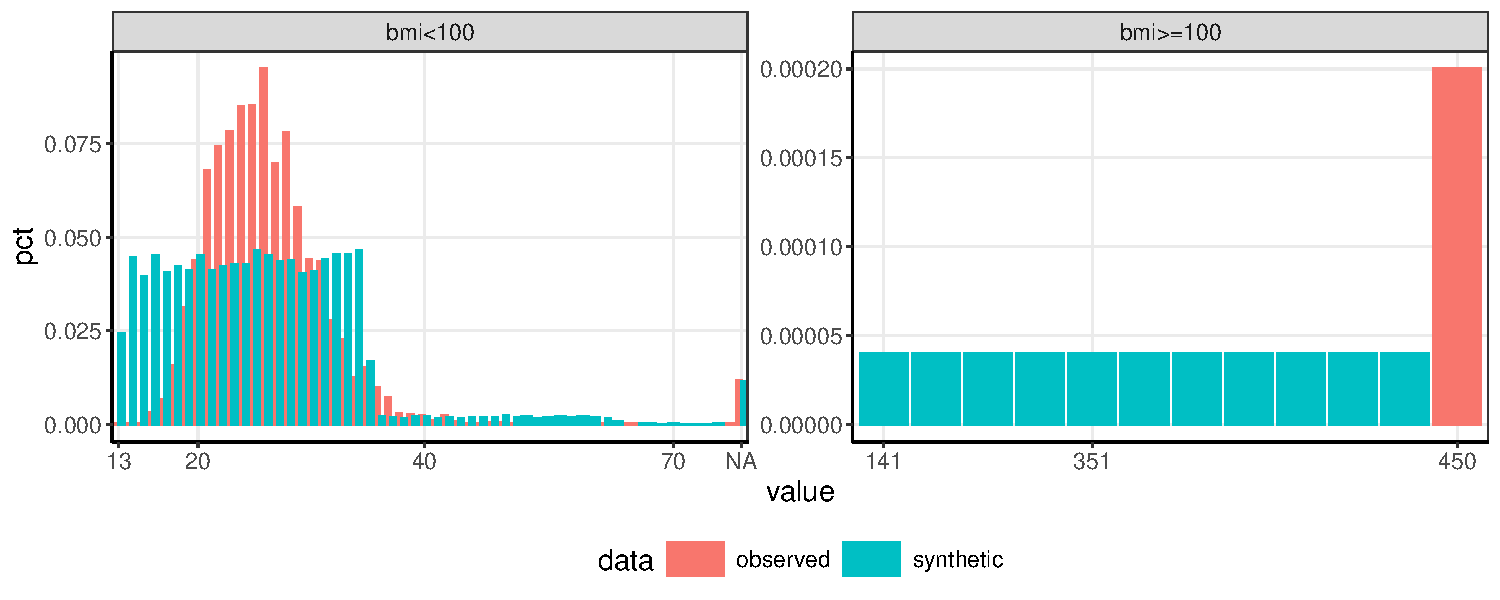
\includegraphics{../graphs/datasynthesizer_bmi.pdf}}
    \caption{Not cleaning the original data can be problematic. For some SDGs the presence of one (unrealistic) outlier leads to synthetic data with many outliers. Here, one false value of the variable body mass index (BMI) leads to a synthetic distribution with many unrealistic values using DataSynthesizer.}\label{fig:graph_datasynthesizer_bmi}
    \vspace{-2em}
\end{figure}

{\bf Messy values.} In real data, variables include messy values, such as spikes in variables that otherwise can be treated as being continuous.  An example in SD2011 is the variable \texttt{nofriend} (number of friends).  In the original data, the variable \texttt{nofriend} appears to be normally distributed below 10, but then clusters at values of 10, 15, 20 and groups of 10 up to the maximum 99.  This phenomenon is sometimes referred to as `spikey', discontinuous, or semi-continuous distributions.  As shown in Figure \ref{fig:graph_datasynthesizer_nofriend} and discussed in more detail below, errors and spikes can pose a problem for statistical utility because most SDGs tend to smooth these spikes unless they are explicitly modeled.

\begin{figure}[t]
    \centering        
    
    \resizebox{.8\textwidth}{!}{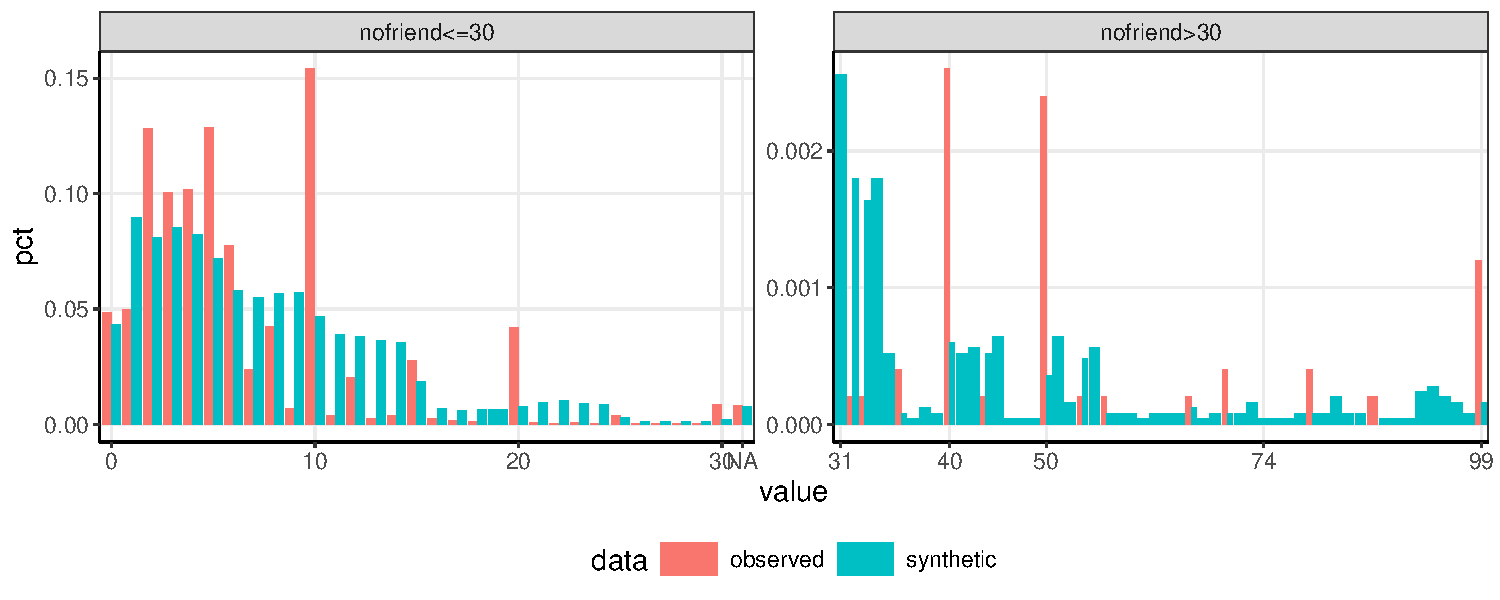
\includegraphics{../graphs/datasynthesizer_nofriend.pdf}}
    \caption{`Spikey', discontinuous, or semi-continuous distributions can be problematic for SDGs. Here, DataSynthesizer seems to smooth spikes in the variable ``Number of friends''.}
    \label{fig:graph_datasynthesizer_nofriend}
    \vspace{-2em}
\end{figure}

To illustrate the importance of pre-processing the data, we use three versions of the original data to create synthetic data and evaluate the utility of each generated dataset using the pMSE.  SD2011(a) is the raw data.  SD2011(b) codes all negative values that indicate missing values in numeric variables and all empty values in character variables as missing.  SD2011(c) drops the two generated variables (\texttt{agegr} and \texttt{bmi}) and then recreates them from the synthetic values. Using DataSynthesizer as our SDG and setting the DAG structure to allow a maximum of two parents, the pMSE changes from 0.2 for SD2011(a) to 0.13 for SD2011(b) to 0.07 for SD2011(c). As measured by the pMSE, the improvements in utility are substantial. In fact, when experimenting with the different tuning parameters of the different synthesizers, we found that none of the tuning parameters had such a strong impact on utility as pre-processing the data (results not reported).   

\section{Know your generator}\label{sec:know_your_generator}

In this section we discuss the importance of knowing the details of the underlying methodology of the SDG to avoid pitfalls or to at least be aware for which analysis tasks the generated data might offer reasonable analytical validity and for which not. We illustrate this point by providing an example of a methodological aspect for each synthesizer that has important impacts on the synthesis, but that might not be immediately obvious when only considering the general methodology of the SDG.  

\subsection{synthpop} 

Categorical variables with large numbers of categories can substantially increase the run-time of CART based synthesizers. To understand why, it is important to understand how CART models are built. CART models operate by finding recursive binary splits to maximize the homogeneity of the values of the dependent variable in the two leaves generated by the split. To find the best possible splits, CART models search over all variables in the dataset. For each variable all possible splits are evaluated and the split that maximizes the homogeneity across all splits and all variables is selected. For continuous and ordered categorical variables the number of splits that needs to be evaluated is $k-1$, where $k$ is the number of unique values in the variable. This is because each value is considered as a possible splitting criteria with all values less than the value ending up in the left leaf and all other values ending up in the right leaf. 

For unordered categorical variables, the number of splits that need to be considered is $2^{L-1}-1$, where $L$ is the number of categories, i.e., the number of splits grows exponentially with the number of categories. To illustrate, imagine one categorical variable with three values (a, b, and c).  There are $2^2-1=3$ possible options to split this variable: (1 = a; 0 = b,c), (1 = b; 0 = a,c), (1 = c; 0 = a,b). With six categories, we already need to consider 31 splits, which still doesn't pose a problem computationally. However, if there are 20 categories, then 524,288 splits need to be considered.  The computational burden can be substantial with even a few categorical variables with a large number of categories.

In the sequential modeling approach that is used with synthpop, each variable that has been synthesized previously is used as a predictor in all subsequent synthesis models.  If a variable with many categories is synthesized early during the synthesis process, it will always be used as a predictor for all other synthesis models imposing a high computational burden on the synthesizer. On the other hand, if the variable is the last variable to be synthesized, it will never be used as a predictor, considerably speeding up the synthesis process. 

For this reason, it is recommended to synthesize categorical variables with many categories last when using CART models \cite{raab2017guidelines}.  However, problems arise if there are a sufficient number of variables with a large number of unique values.  For example, if a Census data set contained variables for 3-digit ISO country code, 3-digit ISCO codes (occupation), and 3-digit ISIC codes (industry), then it would be difficult to avoid computational problems through ordering.  

Other solutions exist, but limitations remain:  One option is to aggregate categorical variables with a large number of unique values.  However, avoiding the information loss from aggregation is typically one of the reasons to rely on synthetic data to begin with.  Alternatively, the categorical variable can be used to stratify the data and to run separate synthesis models within each stratum. Obviously, this will only be an option if the sample sizes in each stratum are still large enough to allow sufficiently rich synthesis models within each stratum.

To illustrate the problem with categorical variables, we examine the duration in time required to create synthetic data using synthpop, i.e. computational efficiency, as shown in table \ref{table:table_sd2011_duration}.  If we load the raw SD2011 into \textsf{R} as a .csv file as we normally do with a SDG, then synthpop requires 2,132 seconds (35 minutes and 30 seconds), but if we load SD2011 into \textsf{R} from the synthpop package, then synthpop requires 5,474 seconds (91 minutes).  The difference in duration within synthpop is explained by two variables: \texttt{eduspec} and \texttt{wkabdur}.  Both variables have a large number of unique values (28 and 33, respectively). Within the synthpop package \texttt{wkabdur} is coded as a character variable, which implies that CART automatically treats it as an unordered categorical variable.  However, if SD2011 is loaded into \textsf{R} from a .csv file, then \texttt{wkabdur} is treated as a numeric variable.  When we treat \texttt{wkabdur} as a numeric variable and place \texttt{eduspec} at the end of the synthesis chain, synthpop requires less than 15 seconds, regardless of how SD2011 is loaded.  

However, the issue reveals a more general problem that synthpop is sensitive to the number (and order) of categorical variables with large values.  To illustrate this, we added one, two, or three categorical variables with 20, 25, or 30 unique random categorical values to the end of the original SD2011 data.  Results are presented in Table \ref{table:table_sd2011_duration}. Duration times for synthpop increase with additional variables and number of unique values.  Table \ref{table:table_sd2011_duration} also reveals that the other synthesizers are less sensitive to the number of categorical variables comprising many categories.

%%%%%%%%%%%%%%%%%%%%%%%%%%%%%%%%
% Tables
%%%%%%%%%%%%%%%%%%%%%%%%%%%%%%%%

\begin{table}[t]
    \centering
    \caption{The effect of data pre-processing on the execution time of the SDGs measured in seconds in wall-clock time. All SDGs were executed on the same machine. }
    \rowcolors{1}{white}{lightgray}
    \resizebox{\textwidth}{!}{% latex table generated in R 4.4.0 by xtable 1.8-4 package
% Fri Jul 19 16:14:31 2024
\begin{tabular}{llrrrr}
  \toprule
version & description & ctgan & datasynthesizer & synthpop (csv) & synthpop (package) \\ 
  \midrule
v00 & Raw (SD2011) & 331.01 & 245.37 & 2132.12 & 5474.39 \\ 
  v01 & Without eduspec or wkabdur & 290.30 & 264.43 & 10.99 & 8.45 \\ 
  v02 & Without wkabdur & 337.07 & 351.76 & 13.96 & 11.02 \\ 
  v03 & Without eduspec & 306.46 & 351.24 & 11.39 & 8.92 \\ 
  v04 & Last variables: eduspec-wkabdur & 374.57 & 344.02 & 14.23 & 287.85 \\ 
  v05 & Last variables: wkabdur-eduspec & 419.60 & 339.92 & 14.60 & 3657.55 \\ 
  v06 & as.numeric(wkabdur) and last variable: eduspec & 356.02 & 347.36 & 14.12 & 11.05 \\ 
  v07\_1\_20 & + 1 factor variable (20 values) & 339.05 & 264.96 & 42.23 &  \\ 
  v07\_1\_25 & + 1 factor variable (25 values) & 400.28 & 326.84 & 137.47 &  \\ 
  v07\_1\_30 & + 1 factor variable (30 values) & 339.73 & 269.72 & 363.18 &  \\ 
  v07\_2\_20 & + 2 factor variable (20 values) & 369.74 & 339.45 & 74.96 &  \\ 
  v07\_2\_25 & + 2 factor variable (25 values) & 364.56 & 361.81 & 631.43 &  \\ 
  v07\_2\_30 & + 2 factor variable (30 values) & 373.25 & 346.15 & 1222.54 &  \\ 
  v07\_3\_20 & + 3 factor variable (20 values) & 393.99 & 369.58 & 122.77 &  \\ 
  v07\_3\_25 & + 3 factor variable (25 values) & 401.03 & 383.40 & 881.53 &  \\ 
  v07\_3\_30 & + 3 factor variable (30 values) & 394.44 & 424.64 & 3654.59 &  \\ 
   \bottomrule
\end{tabular}
}
    \label{table:table_sd2011_duration}
    \\
    \raggedright
    \tiny{Notes: synthpop (csv) indicates that SD2011 was loaded into R from a csv file.  synthpop (package) indicates that SD2011 was loaded into R from the synthpop package.  CTGAN is estimated with 600 epochs.  DataSynthesizer is estimated with two parents.}
    \vspace{-2em}
\end{table}

\subsection{DataSynthesizer}\label{subsec:know_your_generator_datasynthesizer}

The algorithm used by DataSynthesizer assumes that all variables are categorical, like most Bayesian network models \cite{young2009using}.  Making this assumption can simplify the modeling task required to represent complex relationships.  Relatedly, this increases computational efficiency and allows the model to be applied to high dimensional data (see table \ref{table:table_sd2011_duration}) because the information in the data can be reduced without information loss to the full conditional probability table. 

When dealing with continuous variables, Bayesian Networks categorize or discretize these variables prior to estimating the model.  This is done by binning the continuous variable and using the binned variable  for the model.  Once synthetic data have been generated based on this model, values for continuous variables are re-encoded within each bin. Given that the Bayesian Network implicitly assumes conditional independence of the values within a bin and all the other variables contained in the model, it is critical for the analytical validity of the generated data how this encoding step is implemented. DataSynthesizer implements an encoding strategy that samples values from a uniform distribution  within each bin.\footnote{We note that the DataSynthesizer paper states \cite{ping2017datasynthesizer}, ``when invoked in correlated attribute mode, DataDescriber samples attribute values in appropriate order from the Bayesian network.''  However, in the code, it seems that data are created by uniform sampling within a bin (\url{https://github.com/DataResponsibly/DataSynthesizer/blob/90722857e7f6ed736aaa25068ecf9e77f34f896a/DataSynthesizer/datatypes/AbstractAttribute.py\#L125}).  This illustrates the challenge in understanding the methodological details of a given SDG.}  

To demonstrate the consequences of this strategy, we refer to Figures \ref{fig:graph_datasynthesizer_bmi} and \ref{fig:graph_datasynthesizer_nofriend} again, which compare frequency counts for the two variables \texttt{bmi} (body mass index) and  \texttt{nofriend} (number of friends) for SD2011(a), i.e. the raw data.  For  \texttt{nofriend}, DataSynthesizer underestimates the frequencies for small counts and does not preserve the spikes in the data for the larger counts, as it distributes the frequencies equally within the bins. For \texttt{bmi}, synthetic values are not normal as they are in the original data because DataSynthesizer samples from a uniform distribution within the bins.   

\begin{figure}[t]
    \centering        
    
    \resizebox{.8\textwidth}{!}{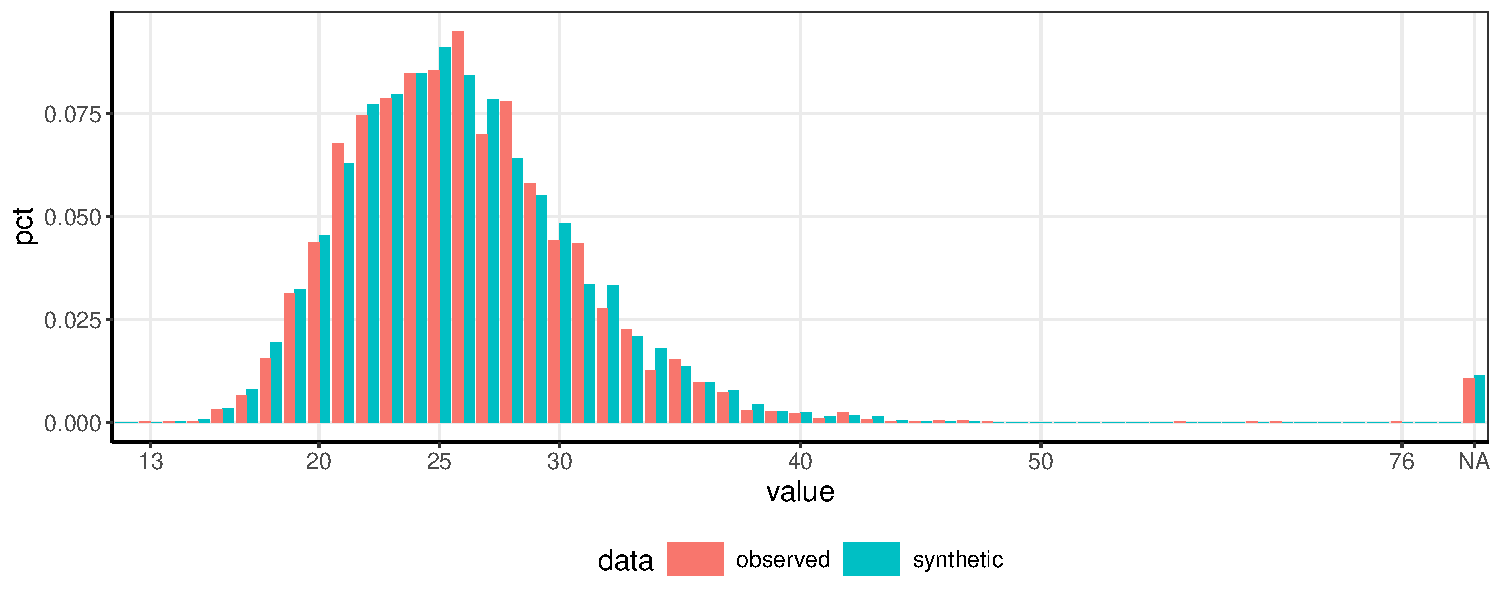
\includegraphics{../graphs/compare_ds_bmi.pdf}}
    \caption{Original and synthetic values of body mass index (BMI) from using DataSynthesizer and the pre-cleaned SD2011(c) dataset.}
    \label{fig:compare_ds_bmi}
    \vspace{-2em}
\end{figure}

However, if we drop \texttt{bmi} before applying DataSynthesizer, and then regenerate \texttt{bmi} from \texttt{height} and \texttt{weight} as we do in SD2011(c), then synthetic values of \texttt{bmi} are  distributed as in the original data, as shown in Figure \ref{fig:compare_ds_bmi}.  While this repeats the importance of cleaning the data prior to applying the synthesizer, this is not a universal solution as the spikiness of \texttt{nofriend} is a feature of the variable that cannot be cleaned.

Of course, the utility of the synthetic data could be improved by increasing the number of bins. However, increasing the number of bins will increase the computational complexity. Besides, setting the number of bins too high would lead to unstable model estimates, as a very large number of parameters would need to be estimated from the data. Furthermore, if the formal privacy guarantees of DataSynthesizer are turned off as in our application, increasing the number of bins can also lead to increased risks of disclosure. If, on the other hand, the formal guarantees should be maintained when increasing the number of bins, more noise needs to be added to each of the parameters and utility would suffer.


\subsection{CTGAN} 

GANs are designed to work well with continuous variables, but GANs can struggle modeling relationships in micro data because cells in micro data are not informative of neighbors in the same way that pixel cells are in a photograph \cite{drechsler202330}.  CTGAN contains a number of hyperparameters that one can use to tune the model.  For this study, we tune the hyperparameters in three main ways.  First, we maintain a constant number of iterations ($3,000$), but allow the batch size to vary, as shown in Figure \ref{fig:ctgan_fidelity_optimize_batch_size}.  Second, we maintain a constant batch size (500), but allow the number of iterations to vary, as shown in Figure \ref{fig:ctgan_fidelity_optimize_epochs}.  Third and finally, we vary the dimensionality of the generator/discriminator networks and the embedding dimension, as shown in Figure \ref{fig:ctgan_fidelity_optimize_dimensions}.  In our data, tuning these hyperparameters makes little difference (pMSE $\approx$ 0.16).  For reference, pMSE from CTGAN is higher than DataSynthesizer (0.07) and synthpop (0.02).

\begin{figure}[t]
    \centering        
   
    \resizebox{.7\textwidth}{!}{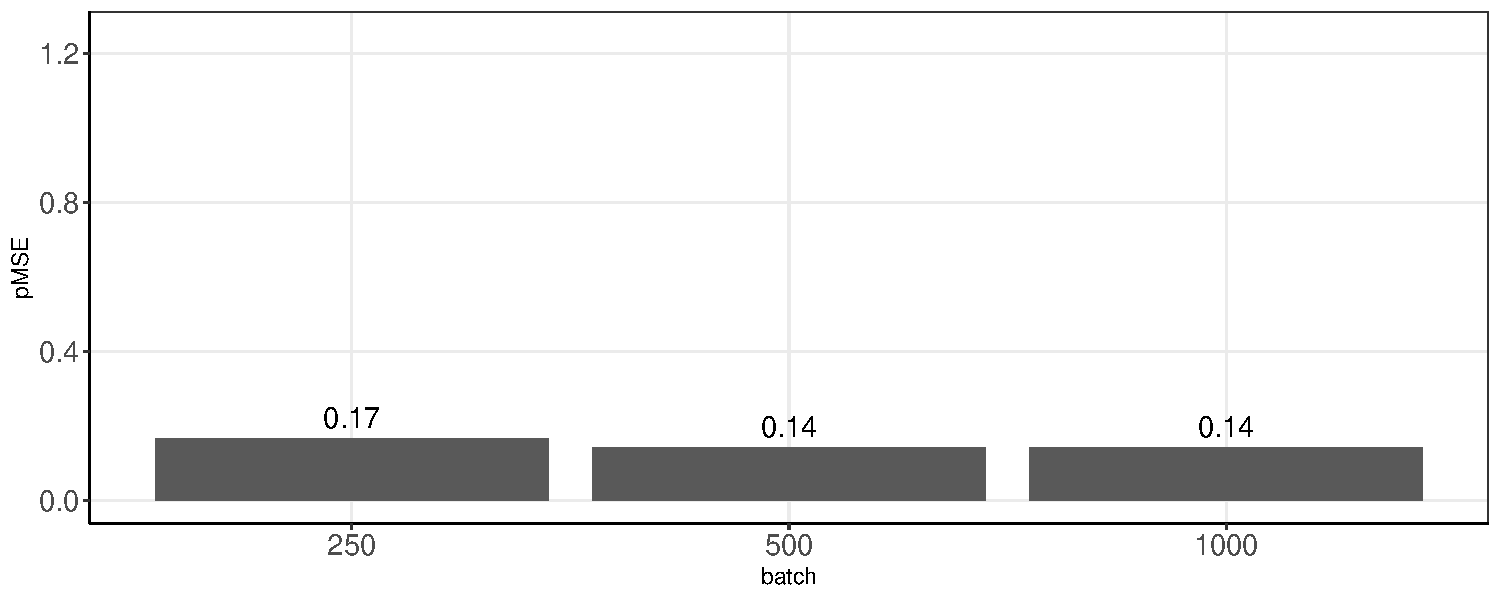
\includegraphics{../graphs/ctgan_fidelity_optimize_batch_size.pdf}}
     \caption{The relationship between batch size and utility of the synthetic data generated by CTGAN (measured by the pMSE) with the number of training steps held constant ($3,000$).}\label{fig:ctgan_fidelity_optimize_batch_size}
     \vspace{-2em}
\end{figure}

\begin{figure}[t]
    \centering        
    
    \resizebox{.7\textwidth}{!}{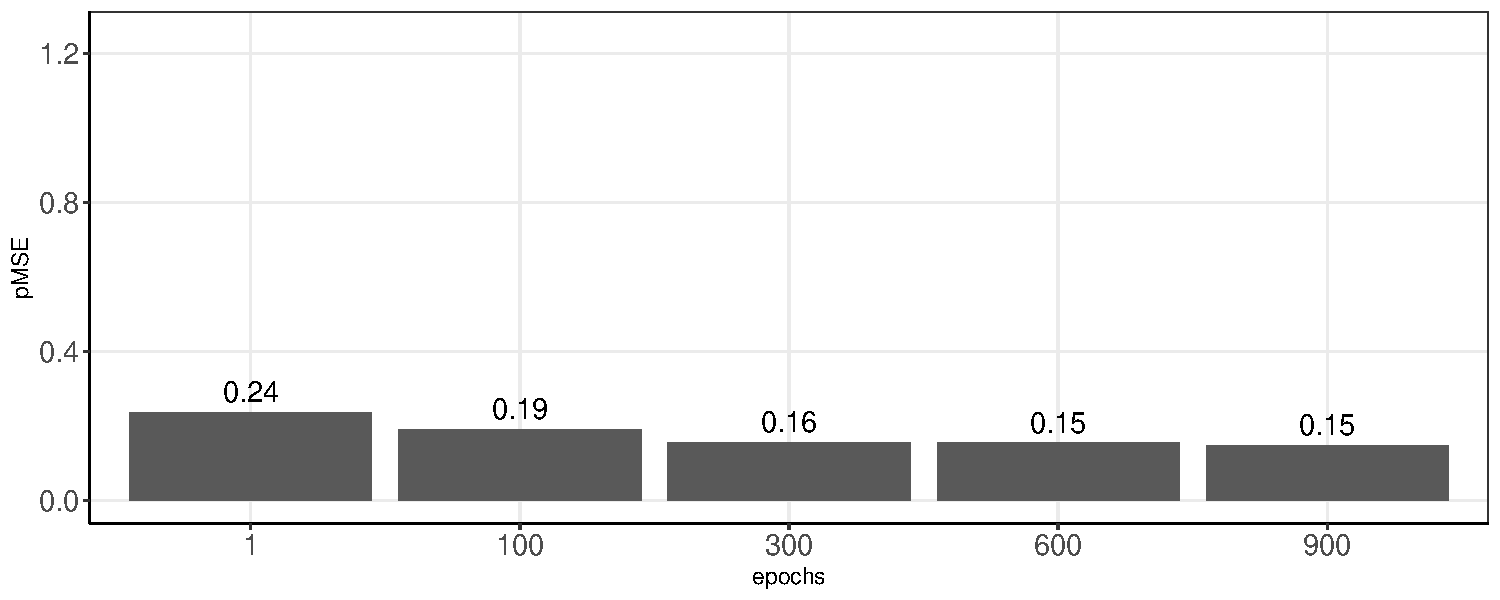
\includegraphics{../graphs/ctgan_fidelity_optimize_epochs.pdf}}
    \caption{The relationship between the number of update steps and utility of the synthetic data generated by CTGAN (measured by the pMSE) with the batch size held constant ($500$).}\label{fig:ctgan_fidelity_optimize_epochs}
    \vspace{-2em}
\end{figure}
    
\begin{figure}[t]
    \centering        
   
    \resizebox{.7\textwidth}{!}{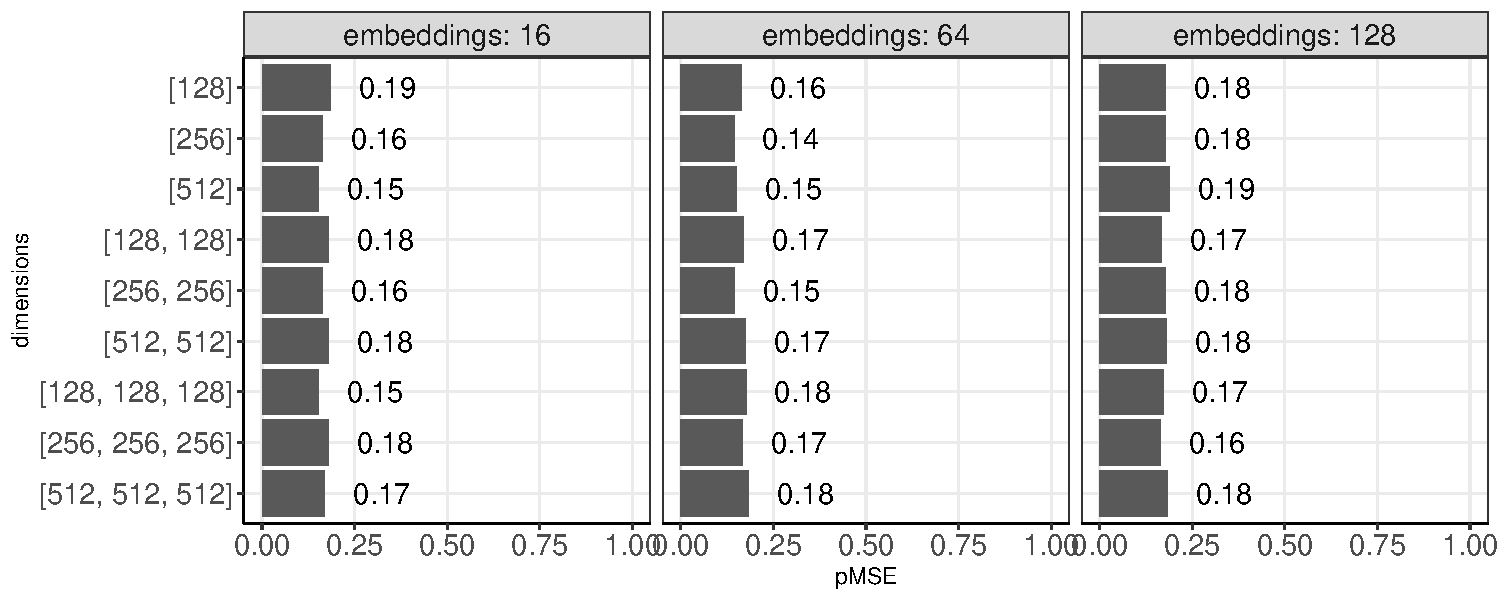
\includegraphics{../graphs/ctgan_fidelity_optimize_dimensions.pdf}}
     \caption{The relationship between the architecture of the CTGAN and utility of the synthetic data (measured by the pMSE).}
     \label{fig:ctgan_fidelity_optimize_dimensions}
     \vspace{-2em}
\end{figure}

We are aware of other research where tuning hyperparameters does make a difference in the quality of synthetic data output (as yet unpublished).  One possible explanation for the fact that hyperparameters do not affect the quality of the synthetic data output is that our data are too low dimensional for the parameters to make a difference.  While CTGAN does not produce data with high levels of utility with the data we use here, we do not mean to suggest that GANs are bad SDGs in general.  CTGAN is not the only GAN in Synthetic Data Vault and multiple other GANs exist. Based on our own experience, it is possible to create a GAN that provides higher levels of utility.  More generally, one must distinguish between the package and the method.  

\section{Conclusion}\label{sec:conclusion}

While generating synthetic data is easier than ever, generating high quality synthetic data remains complicated.  In this article, we make two points.  First, one must know the data.  Most research examining SDGs uses clean data from Census or Machine Learning libraries, especially in the computer science literature.  Unlike clean data, real data contain variables with messy values that can affect the utility of SDGs.  It is not possible to simply input real data into a SDG and expect high quality synthetic data output without carefully pre-processing the data.  The problem is that producing synthetic data with high levels of utility requires knowledge of the data that may not be understood by those with knowledge of the generator.

Second, one must know the generator.  Synthpop produces synthetic data with high levels of utility, but the CART method struggles with computational efficiency on datasets that contain variables with many categories.  DataSynthesizer uses a Bayesian network model to produce synthetic data with high levels of computational efficiency, but the algorithm assumes all variables are discrete, which reduces utility of synthetic continuous variables.  CTGAN uses a GAN architecture to generate synthetic data which may not produce synthetic data with high levels of utility.  There is no one size fits all solution and choosing the right SDG is the result of different trade-offs.  

\begin{credits}
\subsubsection{\ackname} This work was supported by a grant from the German Federal Ministry of Education and Research (grant number 16KISA096) with funding from the European Union—NextGenerationEU.

\subsubsection{\discintname}
The authors have no competing interests to declare that are
relevant to the content of this article.
\end{credits}


%\subsubsection*{Acknowledgments}
%Use unnumbered third level headings for the acknowledgments. All acknowledgments, including those to funding agencies, go at the end of the paper. Only add this information once your submission is accepted and deanonymized. 

%%%%%%%%%%%%%%%%%%%%%%%%%%%%%%%%
% Bibliography
%%%%%%%%%%%%%%%%%%%%%%%%%%%%%%%%
\bibliographystyle{splncs04}
\bibliography{references}

%%%%%%%%%%%%%%%%%%%%%%%%%%%%%%%%
% Appendix
%%%%%%%%%%%%%%%%%%%%%%%%%%%%%%%%

\appendix
\section{Appendix: Utility measures}\label{appendix:utility_measures}
\setcounter{figure}{0}    
\setcounter{table}{0}    

{\bf The propensity score (pMSE)}  is an utility measure that estimates how well one can discriminate between the original and synthetic data based on a classifier \cite{woo2009global,snoke2018general} and is implemented in \textsf{R} from the synthpop package \cite{nowok2016synthpop}.  This is sometimes called a `broad'\cite{snoke2018general} or `general'\cite{drechsler2009disclosure} measure of utility or `statistical fidelity' \cite{jordon2022synthetic}.  The main steps are to append or stack the original and the synthetic data, add an indicator (1/0) to distinguish between the two, use a classifier to estimate the propensity of each record in the combined dataset being `assigned' to the original data. The pMSE is the mean squared error of these estimated propensities:

%%%%%%%%%%%%%%%%%%%%%%%%%%%%%%%%%%%%%%%%%%
\begin{equation}
pMSE = \frac{1}{N}\sum_{i=1}^{N}[\hat{p}_i - c]^2
\end{equation}
%%%%%%%%%%%%%%%%%%%%%%%%%%%%%%%%%%%%%%%%%%
where $N$ is the number of records in the combined dataset, $\hat{p}_i$ is the estimated propensity score for record $i$, and $c$ is the proportion of data in the merged dataset that is synthetic (in many cases $c=0.5$). The pMSE can be estimated using all the variables in the dataset, but it can also be computed using subsets of the variables, e.g., all pairwise combinations of variables to evaluate specifically how well the distribution of these variables is preserved. The smaller the pMSE, the higher the analytical validity of the synthetic data.


{\bf Computational efficiency} is the run time (in seconds) required to create one single synthetic dataset from a given SDG.\footnote{In terms of computing power, SDGs were run on a 2022 Macbook Air with 16GB of RAM and an M2 Chip with 8‑Core CPU, 8‑Core GPU, and a 16‑Core Neural Engine.  All SDGs were run one at a time in order to minimize computational power problems from parallelization.}  This is sometimes referred to as `efficiency'\cite{jordon2022synthetic} or `output scalability' \cite{zhang2017privbayes}.  The basic idea is that the algorithms used by SDGs can suffer from the curse of dimensionality.  

\end{document}
